\section{Exercise 8.14: Smoothing a newspaper picture}

The script \texttt{smooth\_picture.m} reads \texttt{van\_aartsen.jpg} into a matrix $f$ of $M = 894$ by $N = 1192$ pixels and builds a matrix $g$ of the same size whose top-left $L \times L$ pixels are $1$ and all others $0$, with $L = 5$. The smoothed picture follows from the convolution property (8.21), $f ** g = \mathrm{IDFT2}\{F\,G\}$.

\lstinputlisting[caption={MATLAB script \texttt{smooth\_picture.m}}, label={lst:smooth_picture}]{Code/smooth_picture.m}

\subsection*{The spectrum $FG$}

Because $|F|$ spans many orders of magnitude, \cref{fig:smooth-spectra} shows $\log(1 + |F|)$ and $\log(1 + |FG|)$, after \texttt{fftshift} so that $k_x = k_y = 0$ lies in the centre.

\begin{figure}[H]
    \centering
    \begin{subfigure}{0.49\linewidth}
        \centering
        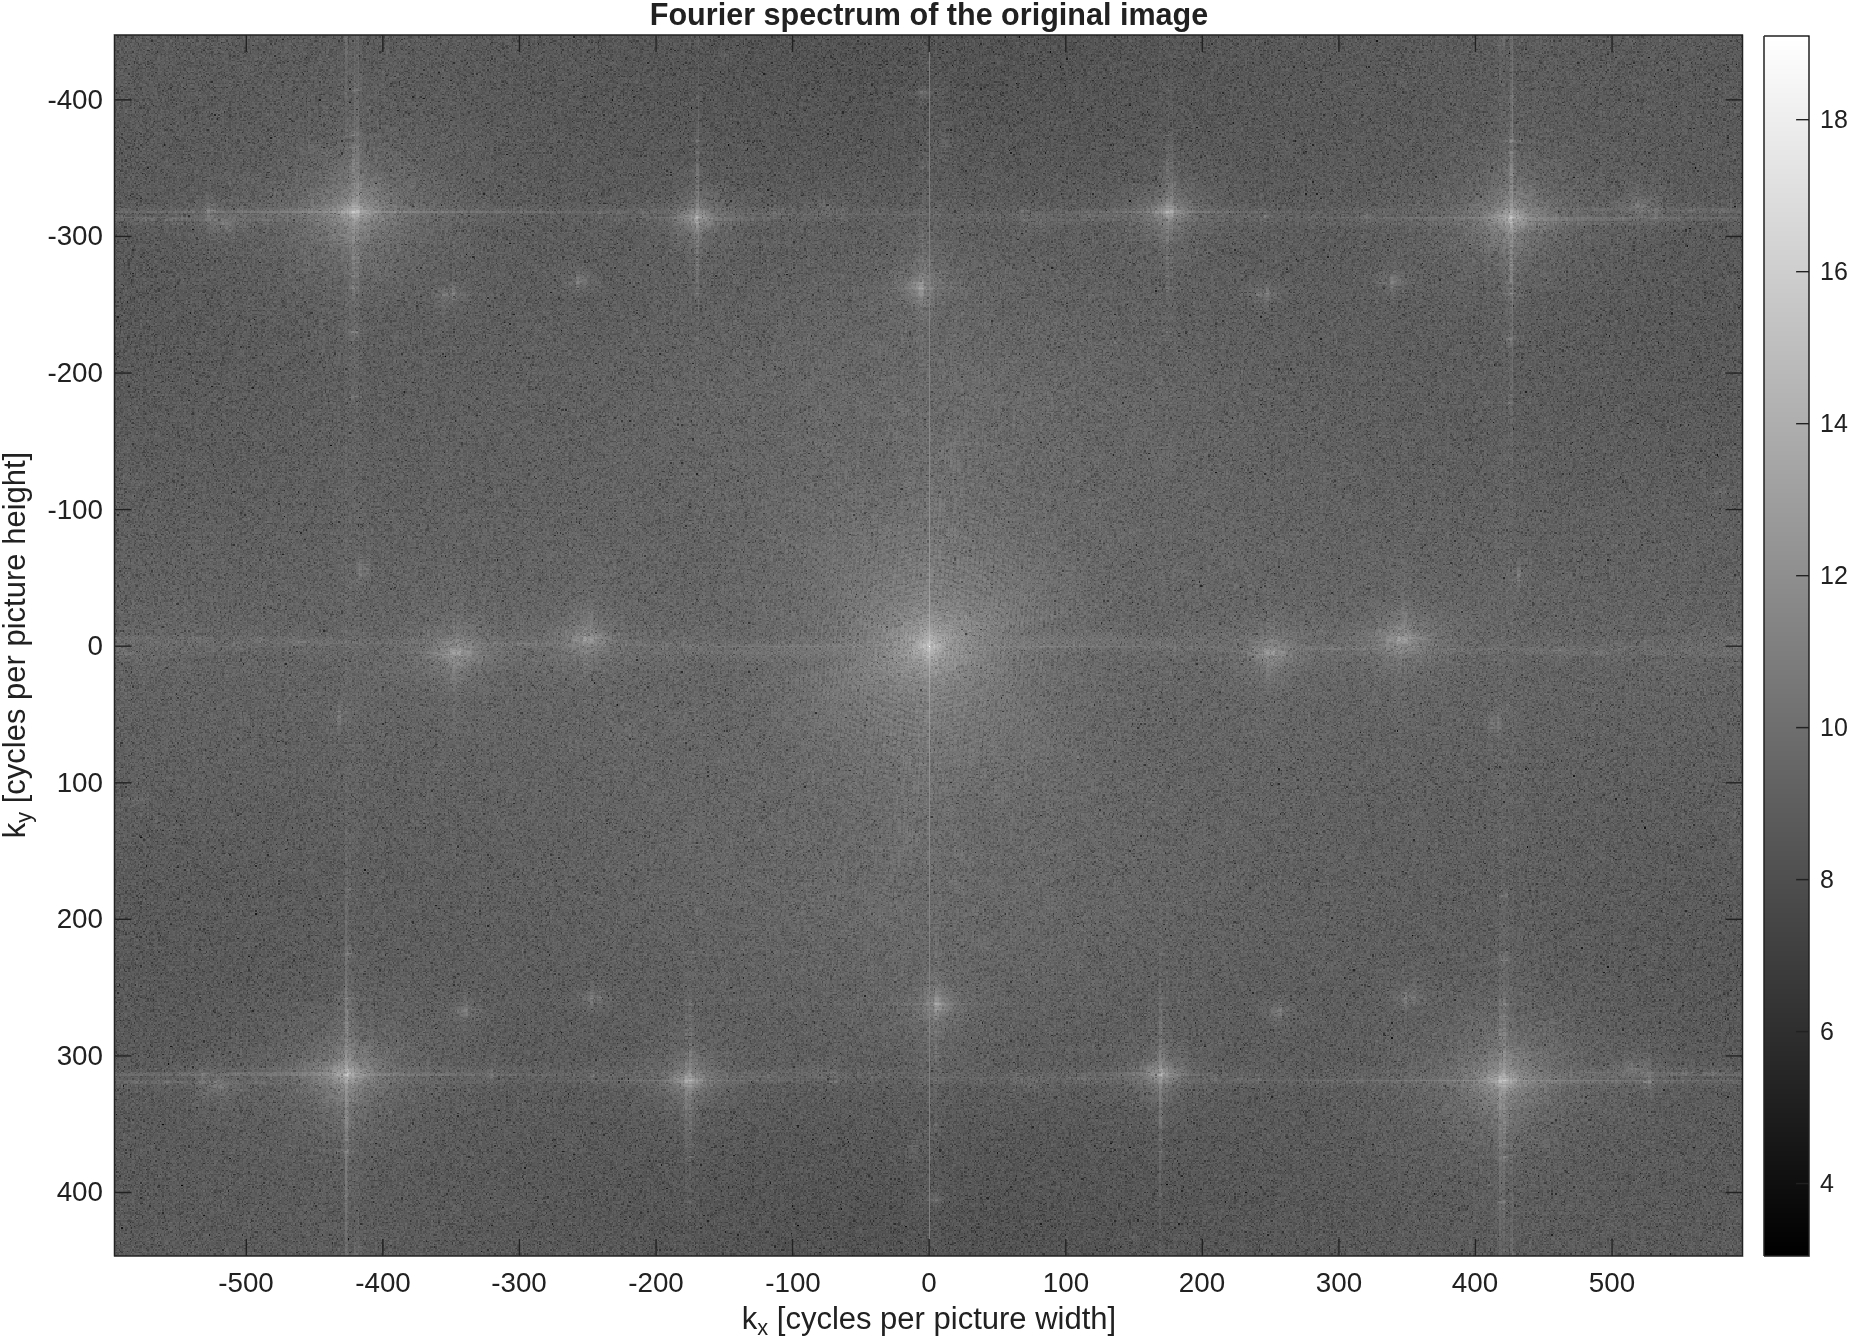
\includegraphics[width=\linewidth]{Figures/smoothing_F_log.png}
        \caption{$\log(1 + |F|)$, original picture}
    \end{subfigure}
    \hfill
    \begin{subfigure}{0.49\linewidth}
        \centering
        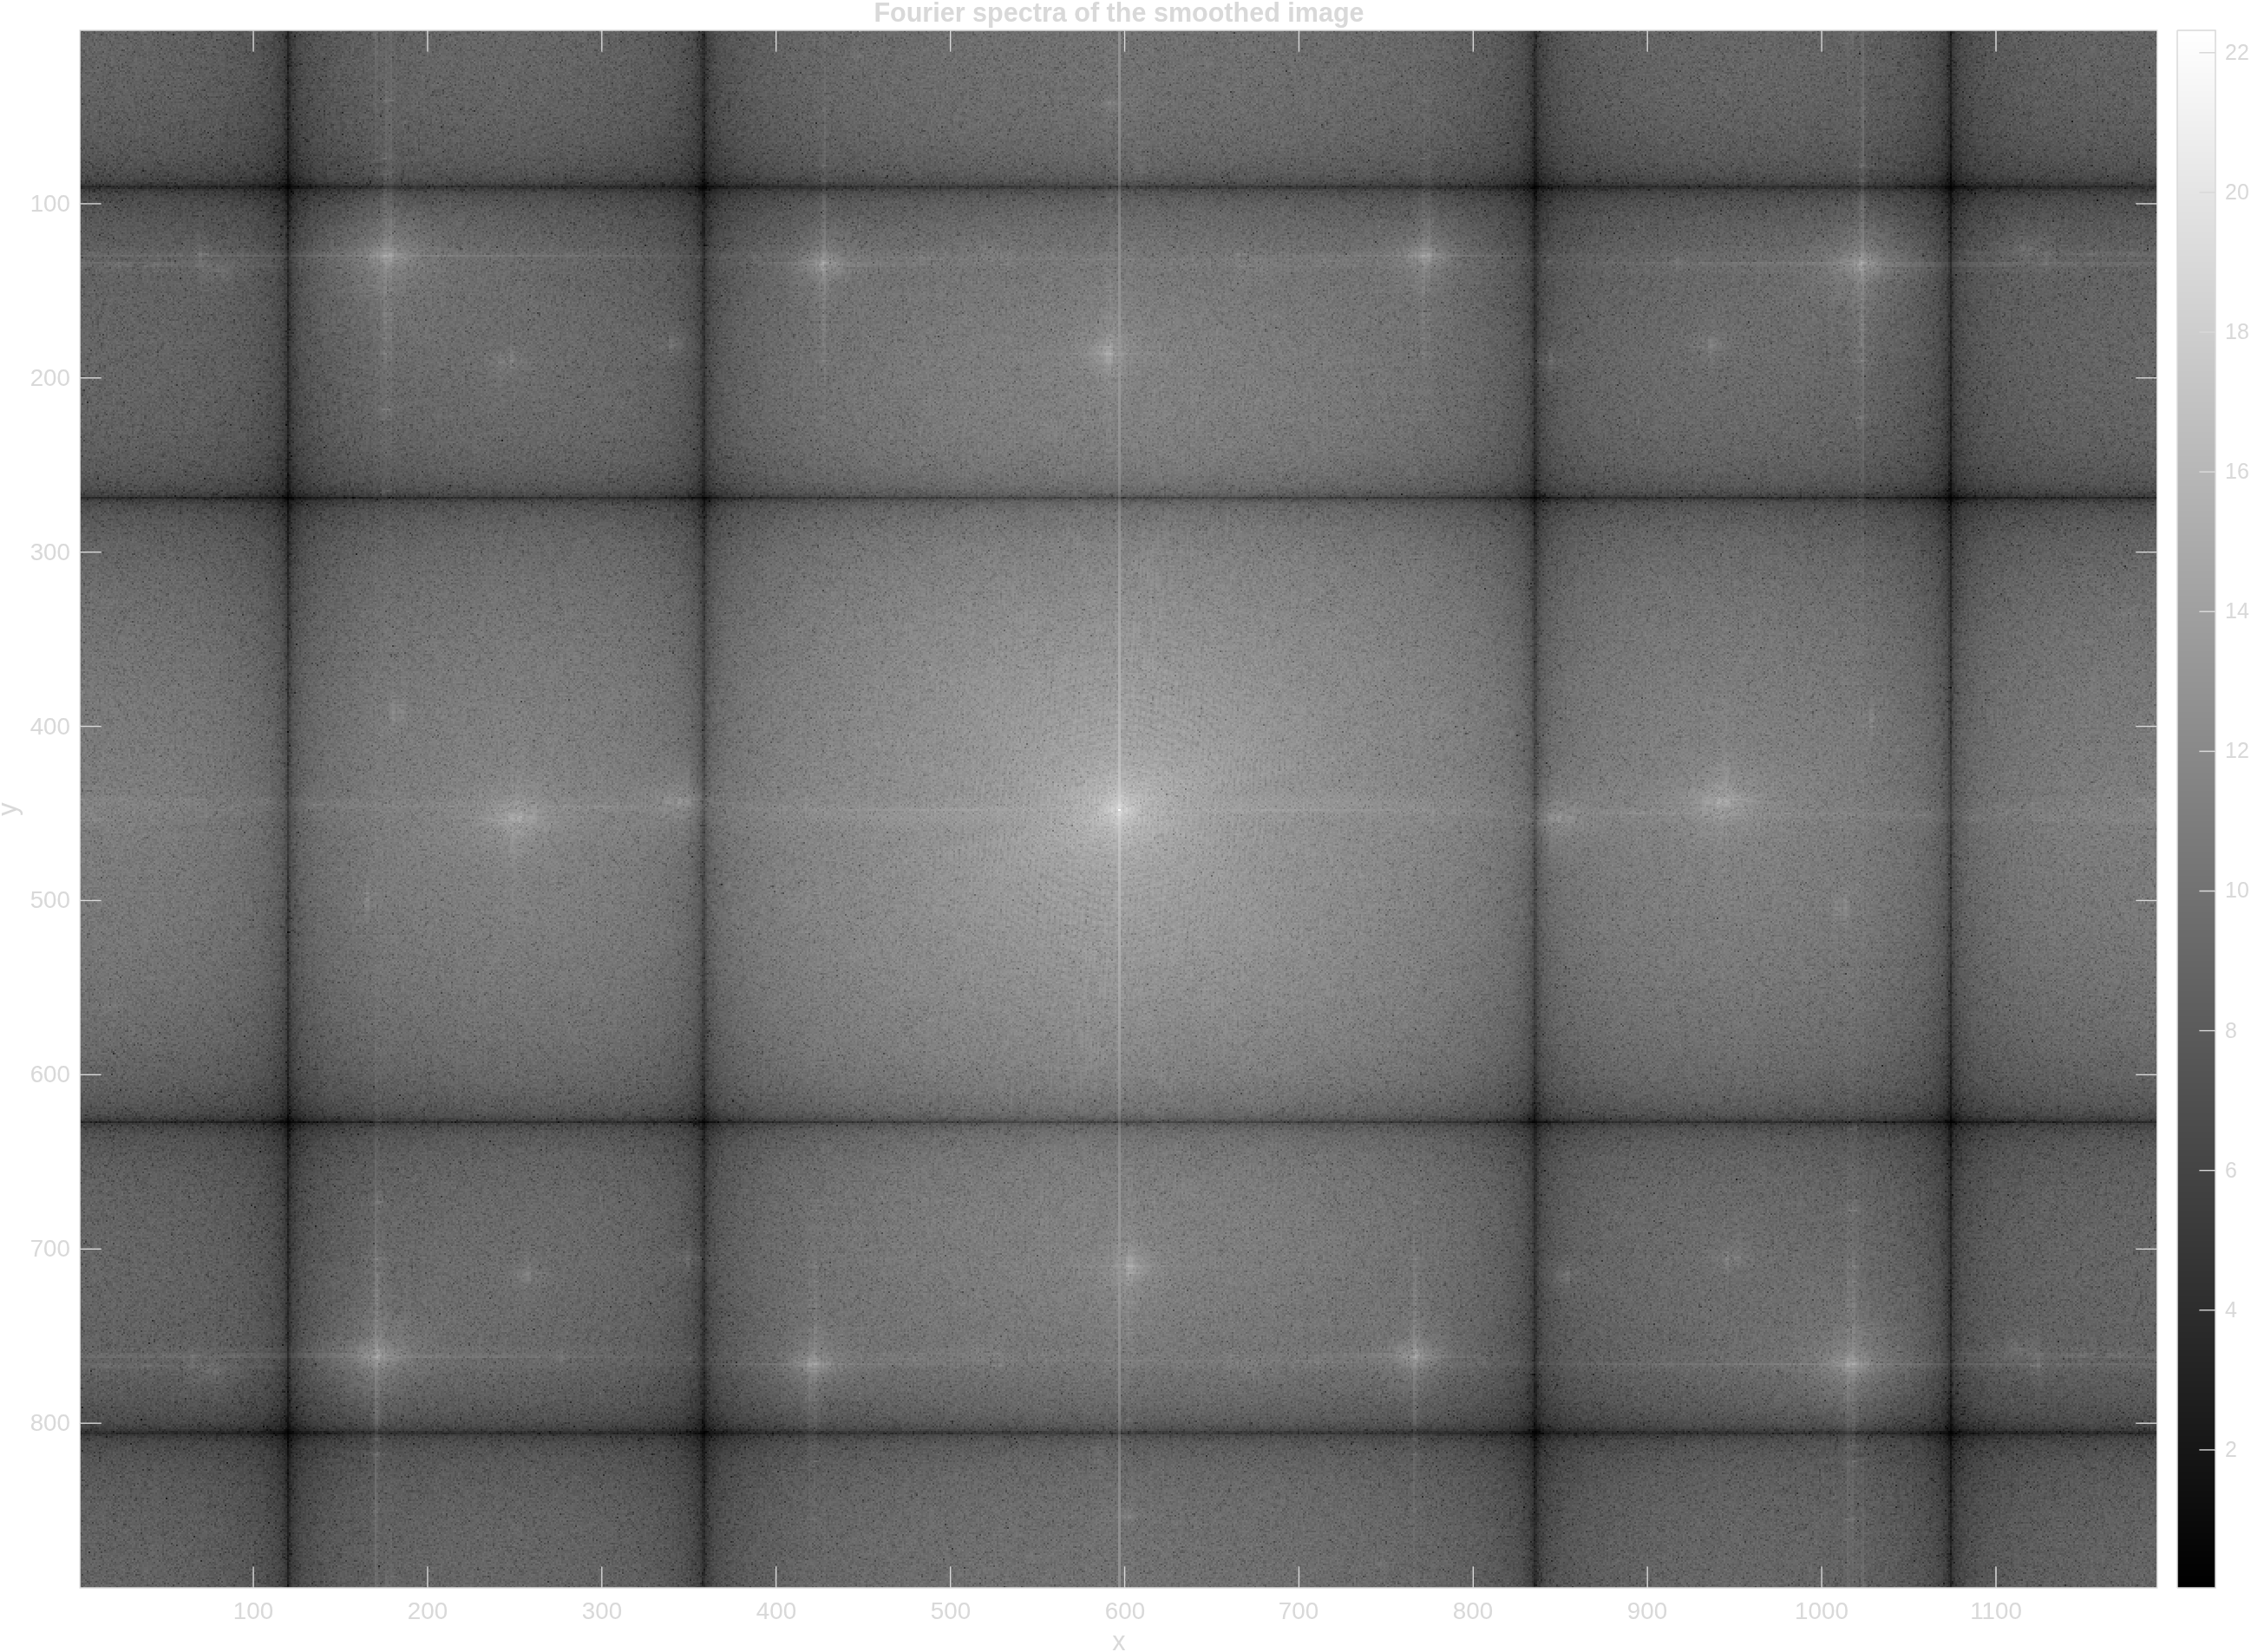
\includegraphics[width=\linewidth]{Figures/smoothing_FG_log.png}
        \caption{$\log(1 + |FG|)$, smoothed with $L = 5$}
    \end{subfigure}
    \caption{Spectra of the original and the smoothed picture, in cycles per picture width and height.}
    \label{fig:smooth-spectra}
\end{figure}

The bright centre of $|F|$ holds the large shapes of the face and background. The regular lattice of peaks further out is the halftone raster of the newspaper print, with a period of about $2.8$ pixels (strongest peaks at $(k_x, k_y) \approx (\pm 426, \pm 314)$). $G$ is the discrete counterpart of a sinc: it is largest at the centre, $G[0,0] = L^2$, and nearly zero at $k_x = p\,N/L$ and $k_y = p\,M/L$ ($p = \pm 1, \pm 2, \dots$), which gives the dark lines in $|FG|$ at $k_x \approx \pm 238$ and $k_y \approx \pm 179$. So $g$ is a low-pass filter: the centre is kept and the raster peaks are reduced by a factor of about $50$.

\subsection*{Original and smoothed picture}

\begin{figure}[H]
    \centering
    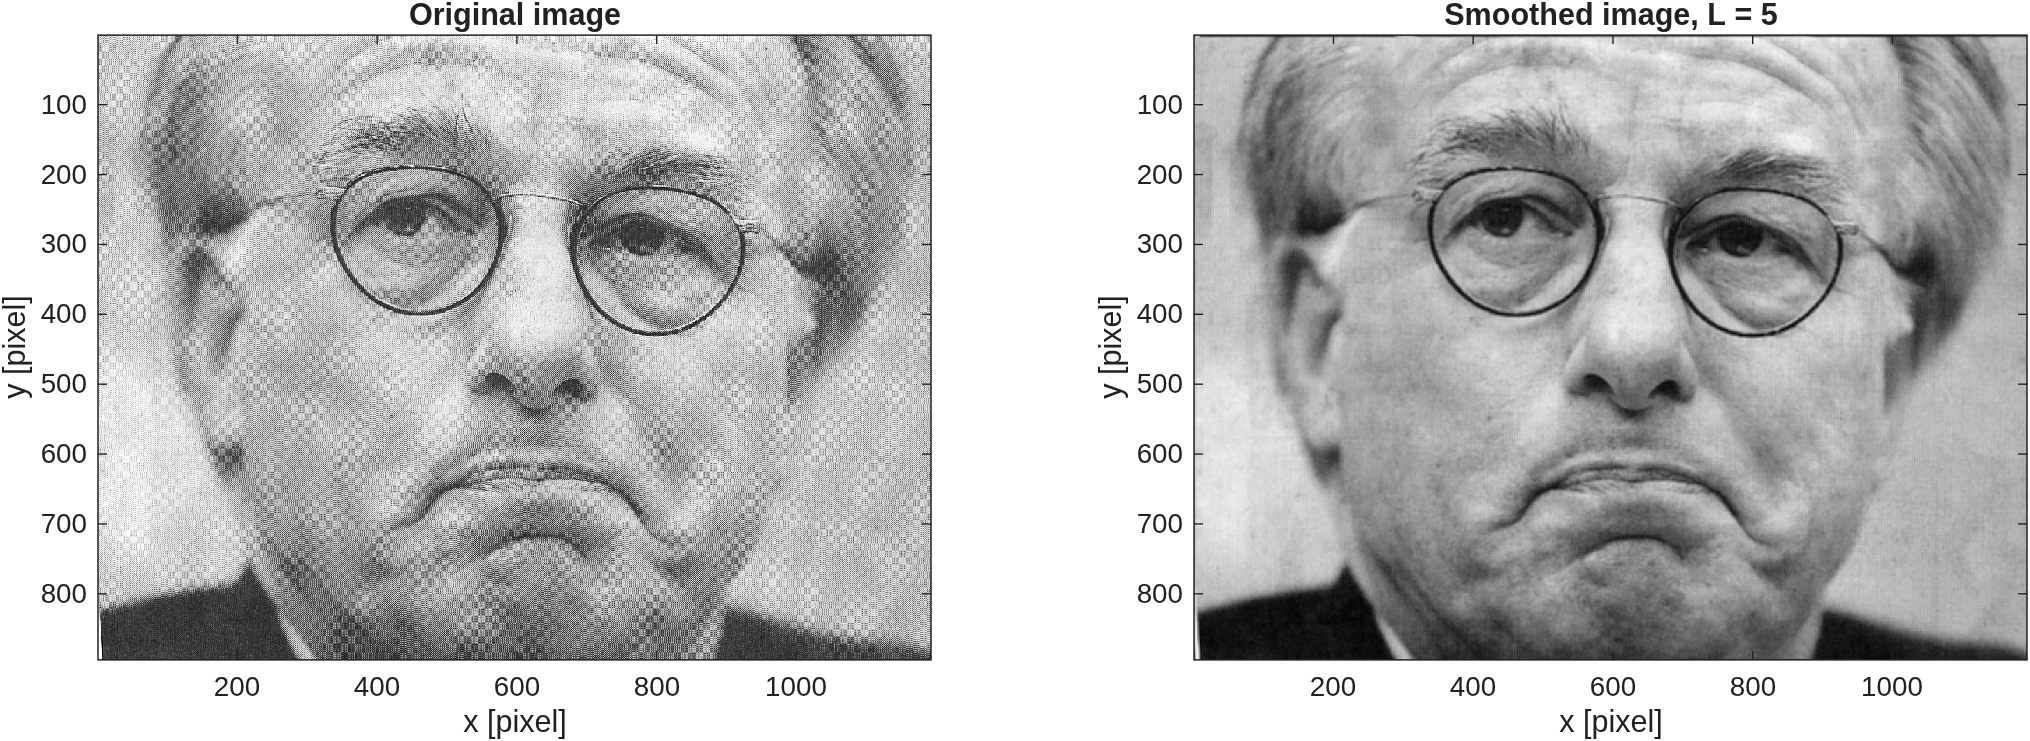
\includegraphics[width=0.85\linewidth]{Figures/smoothing_original_vs_smoothed.png}
    \caption{Original picture (left) and the picture smoothed with $L = 5$ (right).}
    \label{fig:smooth-compare}
\end{figure}

In \cref{fig:smooth-compare} the raster has disappeared, while larger features such as the glasses, eyes and outline of the face remain. Each pixel of $f ** g$ is the sum of the $L \times L$ square that has this pixel as its bottom-right corner. This is the discrete version of exercise 8.2, with three differences: $g$ sums to $L^2$ instead of $1$, so the result is $L^2$ times the average (not visible, because \texttt{imagesc} rescales the colours); the square is not centred on the pixel, which shifts the picture by $(L-1)/2$ pixels; and the DFT treats the picture as periodic, so squares at the top and left edges take pixels from the opposite edges. Away from those edges the result agrees with the direct convolution \texttt{conv2(f, ones(L))} to within $1.3 \cdot 10^{-11}$.

\subsection*{Influence of $L$}

\begin{figure}[H]
    \centering
    \begin{subfigure}{0.32\linewidth}
        \centering
        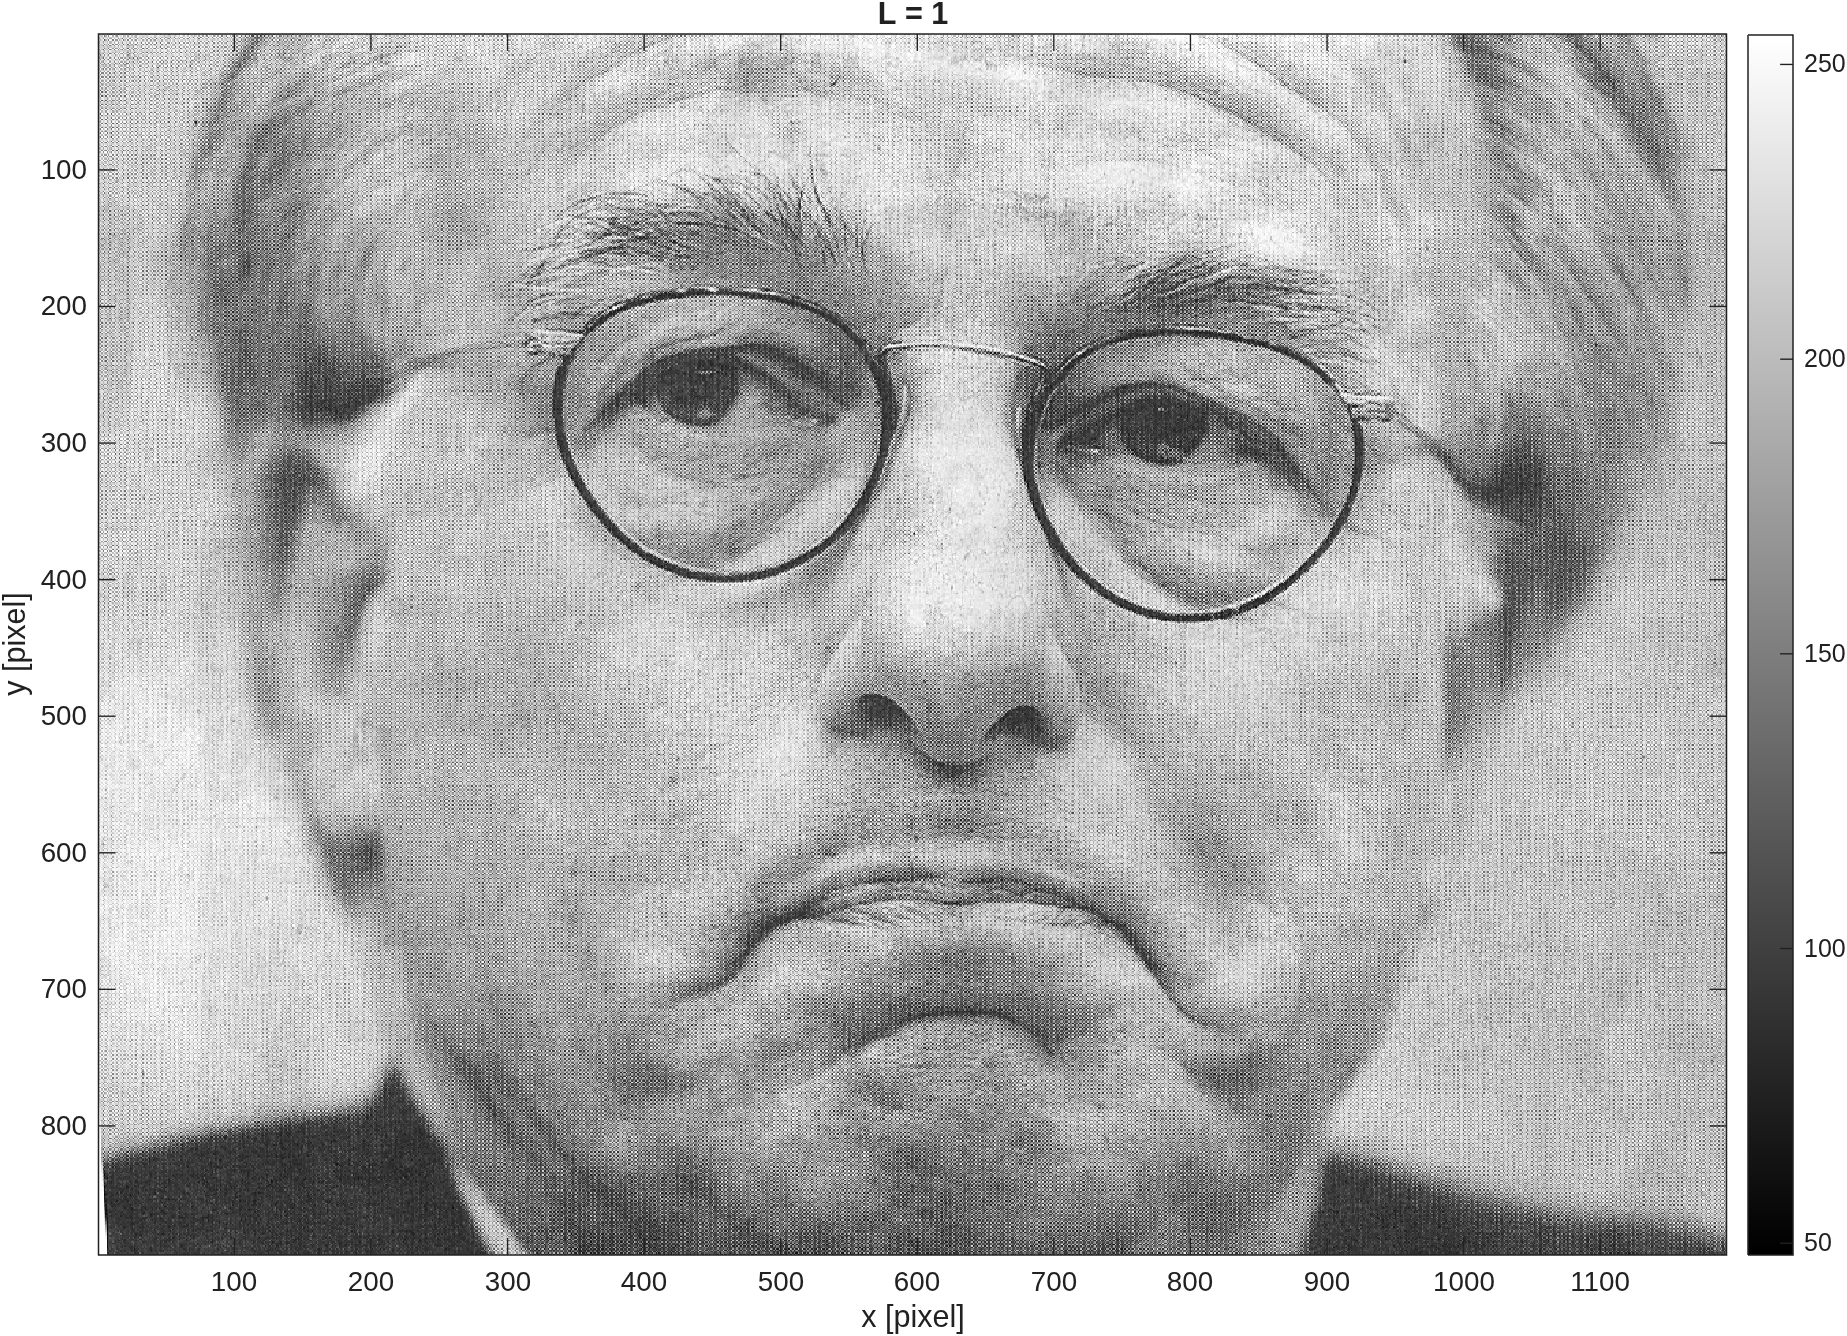
\includegraphics[width=\linewidth]{Figures/smoothing_f_convolution_L1.png}
        \caption{$L = 1$}
    \end{subfigure}
    \hfill
    \begin{subfigure}{0.32\linewidth}
        \centering
        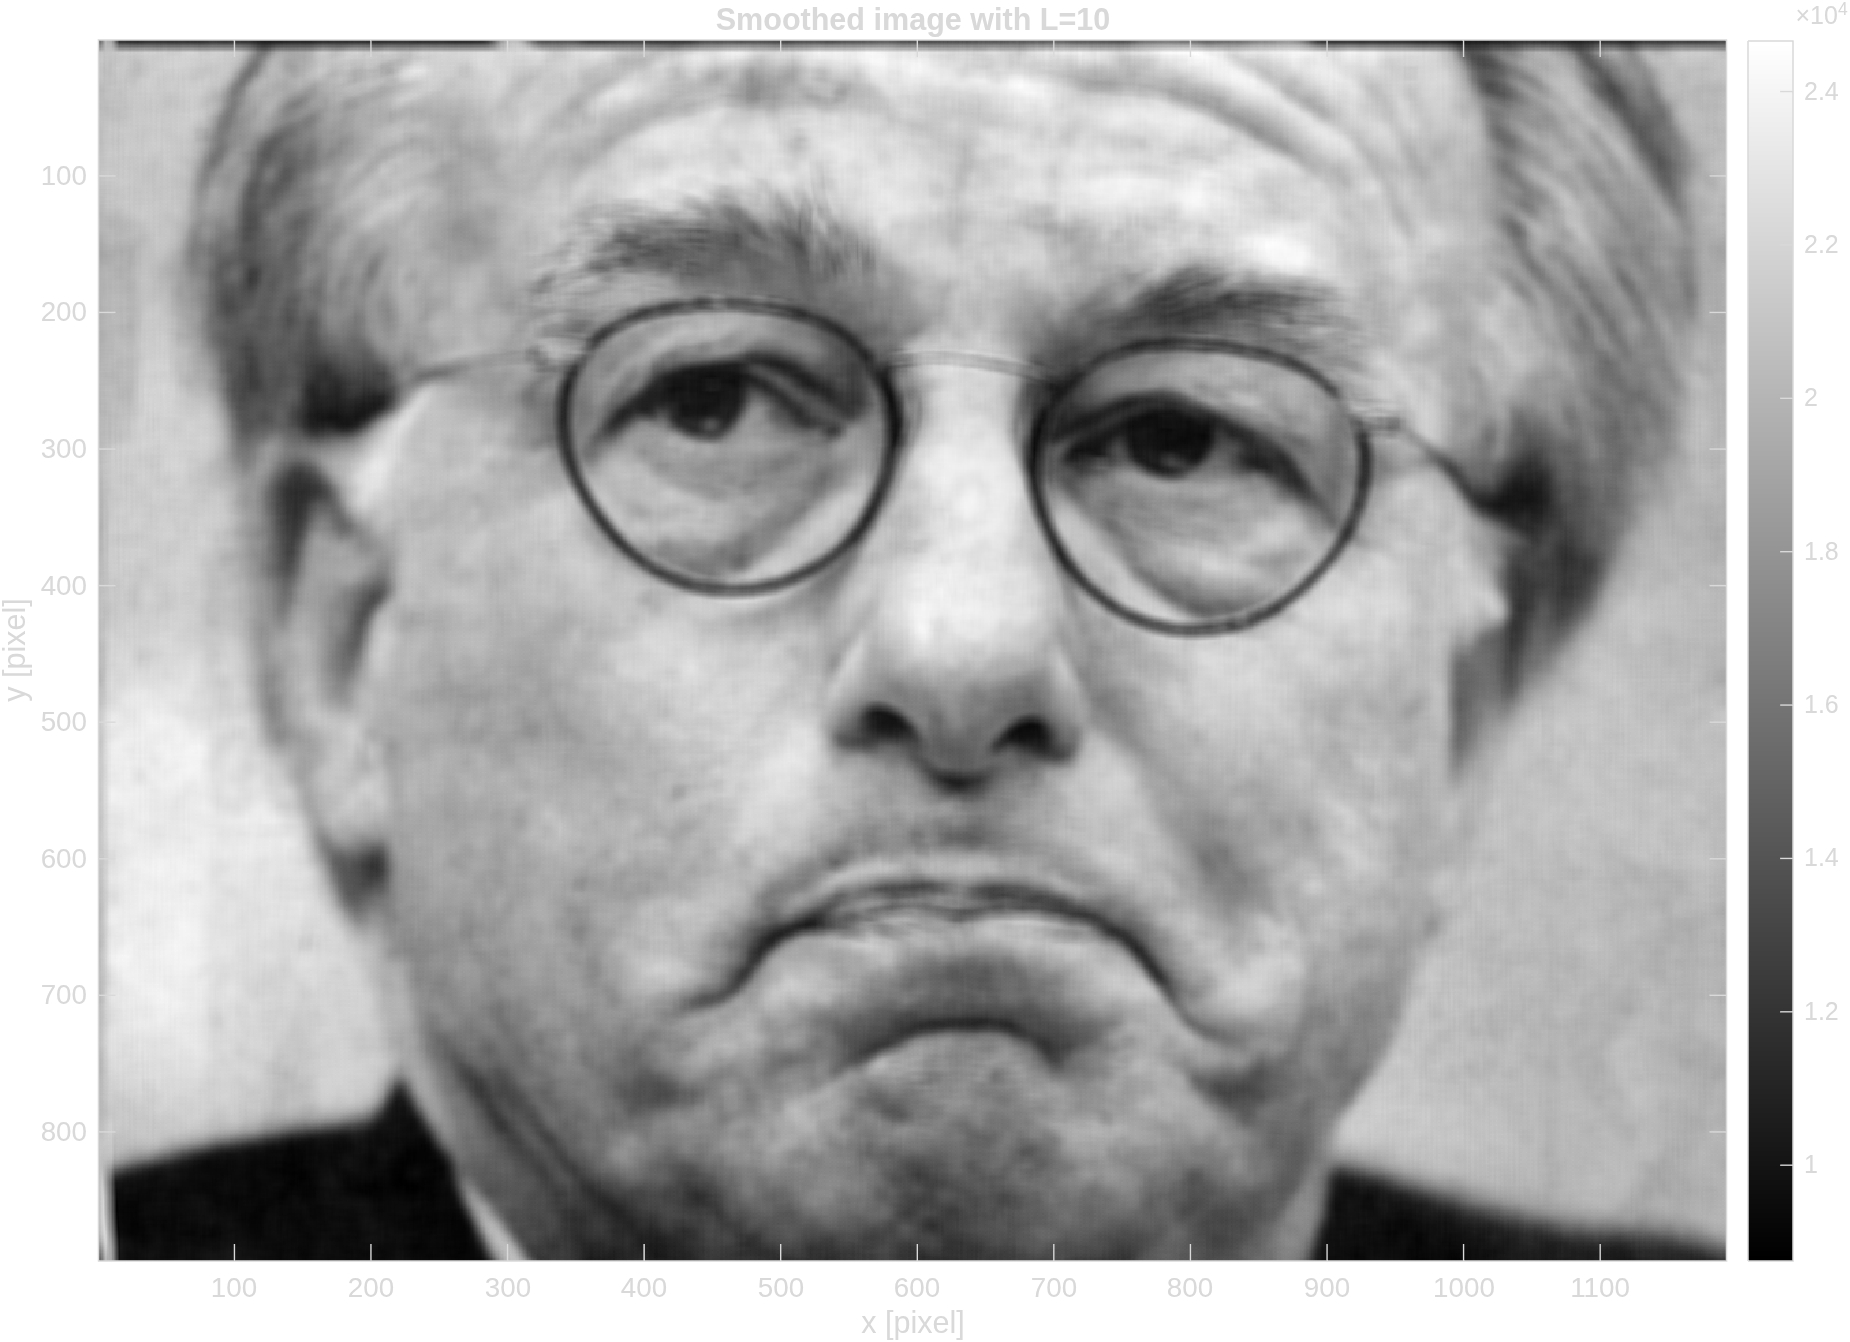
\includegraphics[width=\linewidth]{Figures/smoothing_f_convolution_L10.png}
        \caption{$L = 10$}
    \end{subfigure}
    \hfill
    \begin{subfigure}{0.32\linewidth}
        \centering
        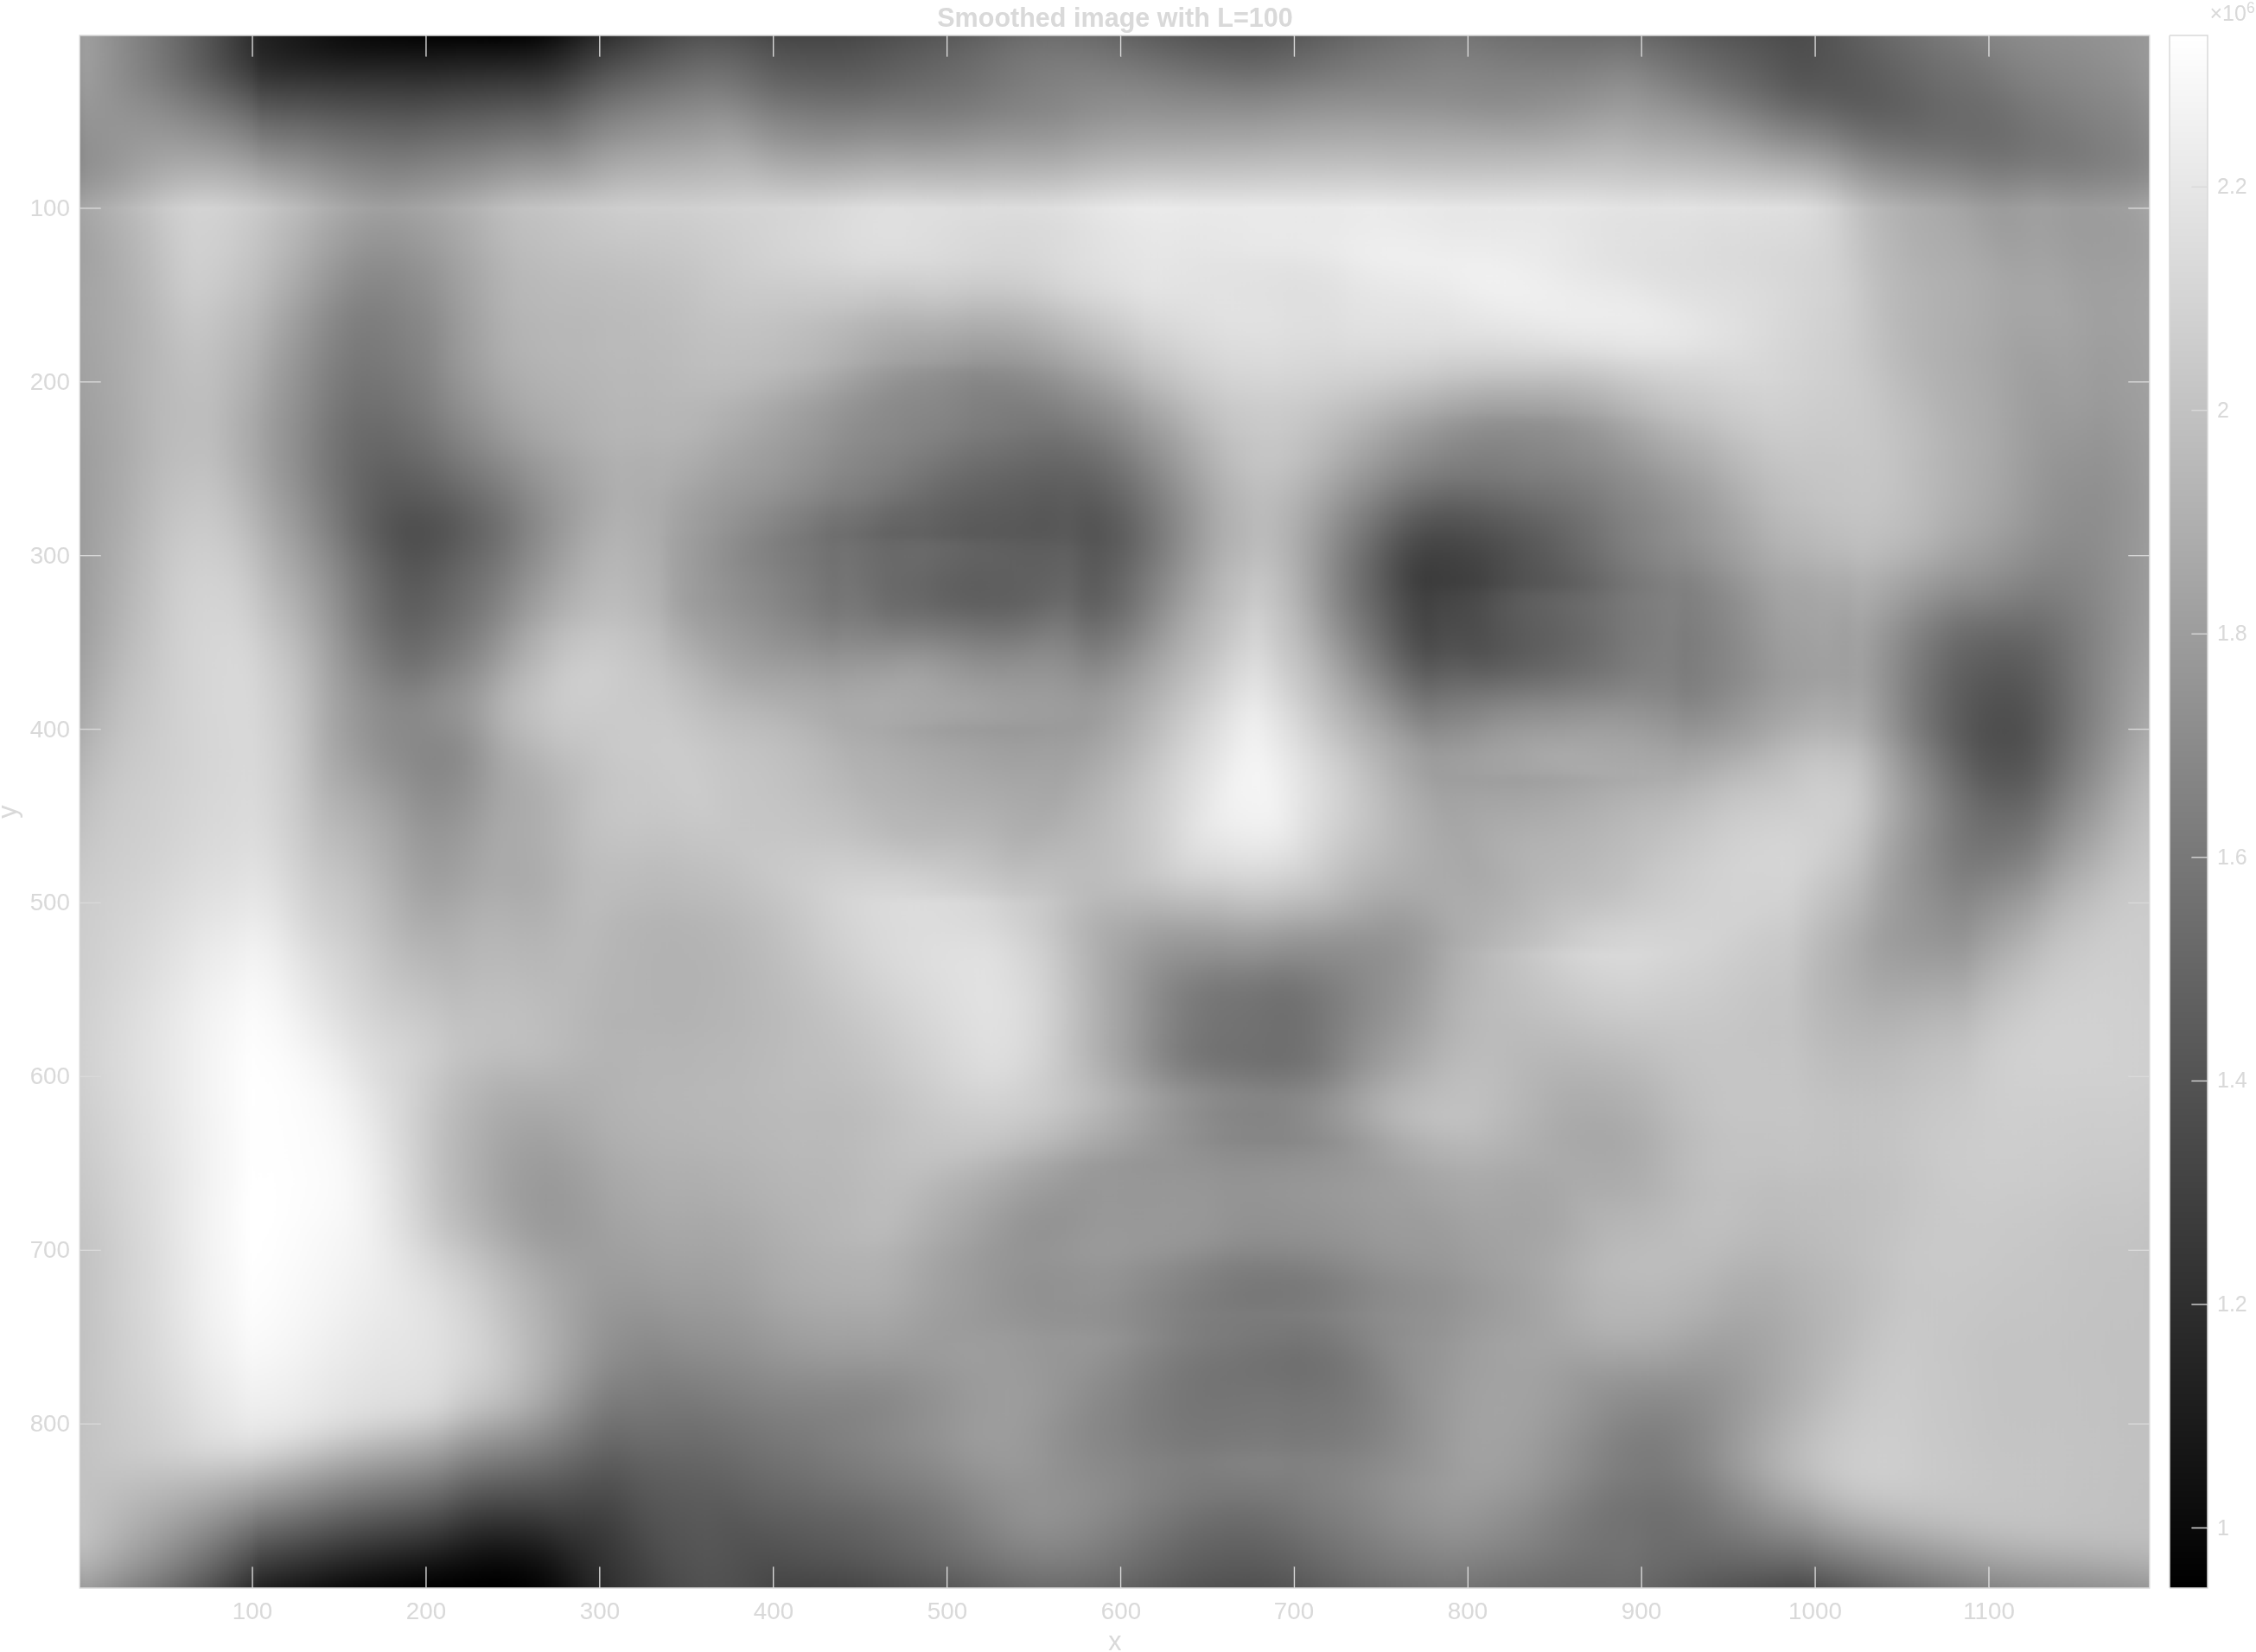
\includegraphics[width=\linewidth]{Figures/smoothing_f_convolution_L100.png}
        \caption{$L = 100$}
    \end{subfigure}
    \caption{The picture convolved with an $L \times L$ block of ones.}
    \label{fig:smooth-L}
\end{figure}

The band of frequencies that $G$ passes shrinks as $1/L$ (\cref{fig:smooth-L}). A larger $L$ removes more of the raster but also more detail: for $L = 100$ only the coarse shapes remain, the picture is shifted by about $50$ pixels, and a dark band appears along the top edge because those squares wrap around to the dark jacket at the bottom. A smaller $L$ keeps more detail but removes less of the raster. For $L = 1$, $g$ is a discrete delta peak, so $G = 1$ and $f ** g = f$ (relation 8.5); the computed result equals the original up to $6.8 \cdot 10^{-13}$. $L = 5$ spans almost two raster periods and is a good compromise.
